%!TEX root = FreeRtos ARM uController.tex
\subsection{Einrichten und Konfiguration}
\label{sec:Einrichtung und Konfiguration}
Dieser Abschnitt beschreibt die Einrichtung eines FreeRTOS Projektes für den STM32F4. Die Beschreibung dabei ist nicht vollständig und versteht sich eher als eine Art Leitfaden. Alle anwendungsspezifischen Konfigurationen können in den zur Verfügung gestellten Links nachgelesen werden. Hierbei ist besonders die Seite des GNU ARM Plugins hervorzuheben, da diese einen guten Einstieg für die Erstellung eines ARM Projekts bietet. Als Entwicklungsumgebung wird Eclipse CDT verwendet, welches bereits in Abschnitt \ref{ref:Entwicklungsumgebung} beschrieben wurde. Nach der Installation von Eclipse muss das GNU ARM Plugin für Eclipse CDT installiert werden. Dies ist entweder über den Pluginmanager oder über den folgenden Link erhältlich: 
\newline
\newline
http://gnuarmeclipse.github.io/
\newline
\newline
Das Plugin ermöglicht die Einbindung und die Konfiguration von ARM Cross Compilern. Des Weiteren stellt es einige Beispielprojekte für ARM uController zur Verfügung. Nach der Installation des ARM Plugins, müssen die GCC ARM Toolchain und die GNU Build Tools installiert werden. 
Diese könne hier heruntergeladen werden: 
\newline
\newline
https://launchpad.net/gcc-arm-embedded
\newline
https://github.com/gnuarmeclipse/windows-build-tools/
\newline
\newline
Die Toolchain und die Buildtools stellen nötigen Anwendungen die zum Compilieren und Debuggen der C und C++ Dateien benötigt werden. Zur Toolchain gehören unter anderem GCC als Cross Compiler und GDB (GNU Debugger) zum Debuggen der Anwendung auf der Zielplattform. GNU Buildtools beinhalte make und rm, die zum Organisieren des Builds benötigt werden. Nach der Installation müssen die Verzeichnisse der Toolchain und der Buildtools im Plugin konfiguriert werden. Mit dieser Konfiguration ist das System nun in der Lage C und C++ Dateien für die Zielplattform zu kompilieren und als Binary File (.elf) bereitzustellen. Zum Übertragen und Debuggen der Anwendung auf dem Zielsystem wird ein ISP-Programmer für ARM benötigt.\needspace{5\baselineskip} Folgende ISP-Programmer werden häufig verwendet, dabei ist Liste weder vollständig, noch stellt eine Empfehlung dar.
\begin{itemize}
	\item Segger J-Link:
	\newline
	https://www.segger.com/jlink-debug-probes.html
	\item Keil Ulink: 
	\newline
	http://www2.keil.com/mdk5/ulink
	\item STM ST-Link/VL: 
	\newline
	http://www.st.com/en/development-tools/st-link-v2.html
\end{itemize}
Zur Nutzung des ISP müssen die benötigten Treiber und der On-Chip Debugger des Herstellers installiert werden. Eine Alternative zum On-Chip Debugger des Herstellers ist OpenOCD. Details dazu findet man unter:
\newline
\newline
http://openocd.org/
\newline
\newline            
Nachdem die Konfiguration der Entwicklungstools abgeschlossen ist, kann nun eine Basis Projekt erstellt werden. Hierfür verwendet man am Besten ein Templateprojekt des GNU ARM Plugins, siehe Abbildung \ref{fig:NewProj}.
\begin{figure}[htb]
	\centering
		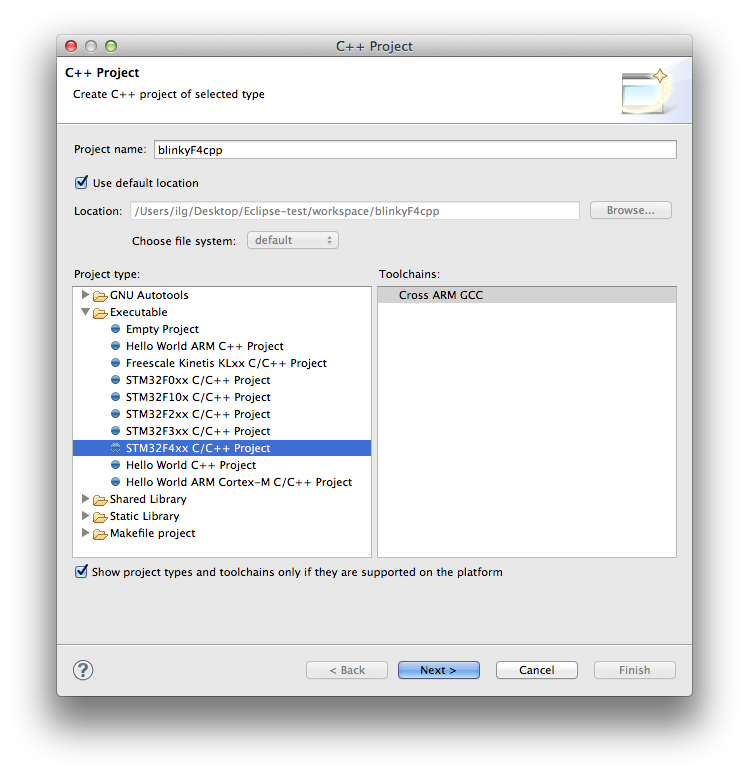
\includegraphics[width=0.4\textwidth]{Pictures/Einrichtung/NewF4Project.png}
	\caption{Erstellung eines Basisprojekts für den STM32F4 durch das GNU ARM Plugin. Ein Wizzard Konfigurator führt den Anwender durch alle nötigen Einstellungen. Nach Abschluss erhält man ein fertiges C / C++ ARM Projekt welches passend zum Zielsystem konfiguriert ist.}
	\label{fig:NewProj}
\end{figure}
Das Templateprojekt beinhaltet bereits alle benötigten Hardware Librarys (Abbildung \ref{fig:CMSIS}) wie die STM HAL (siehe Abschnitt \ref{sec:Zielsysteme}) oder das ARM CMSIS (Cortex Microcontroller Software Interface Standard).
\begin{figure}[htb]
	\centering
		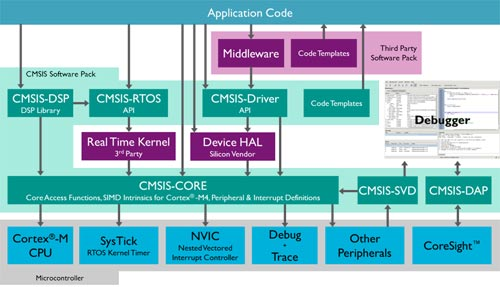
\includegraphics[width=0.4\textwidth]{Pictures/Einrichtung/CMSISv4_small.jpg}
	\caption{ARM embedded Anwendungen setzten auf unterschiedliche Abstraktionsschichten auf. Die untersten beiden Abstraktionsschichten sind CMSIS, welches Funktionen für ARM Devices bereitstellt und die HAL des uController Herstellers. CMSIS steht für alle ARM Systeme zur Verfügung, wohingegen die HAL uController spezifisch ist. }
	\label{fig:CMSIS}
\end{figure}
Das Templateprojekt sollte jetzt kompilieren und mittels ISP-Programmer auf auf dem Zielsystem ausgeführt werden können.
Im nächsten Schritt wird FreeRTOS in das Templateprojekt eingebunden. Hierfür kann auf www.freertos.org die gepackte Variante der Demoprojekte heruntergeladen werden. Für den STM32F4 stehen spezielle Cortex M4 Portierungen zur Verfügung. Die Verzeichnisstruktur sollte dabei der Abbildung \ref{fig:SourceTree} ähneln.
\begin{figure}[htb]
	\centering
		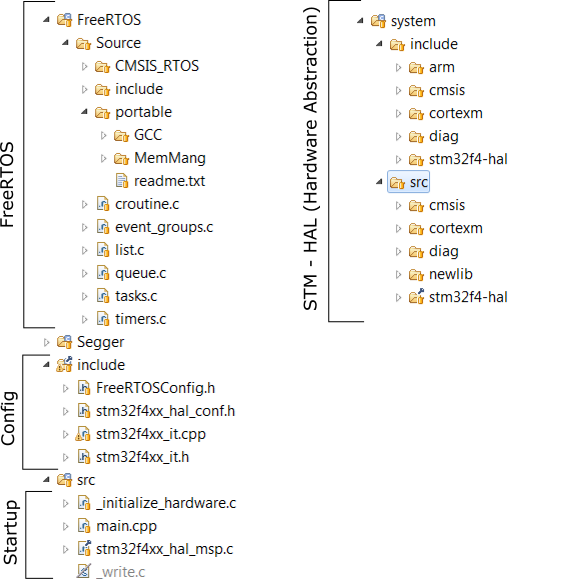
\includegraphics[width=0.4\textwidth]{Pictures/Einrichtung/sourceTree.png}
	\caption{Die Basiskonfiguration die durch das GNU ARM Plugin zur Verfügung gestellt wird, besteht aus den Verzeichnissen: Startup, Config und HAL. Startup beinhaltet alle Files zum Starten der Hardware und die main. Im Config Verzeichnisse befinden sich alle Files zur Konfiguration des uControllers und die FreeRTOS Config. Die HAL und CMSIS sind die Grundlage des Systems und werden ebenfalls durch das GNU ARM Plugin eingefügt. FreeRTOS wird danach manuell dem Projekt hinzugefügt.}
	\label{fig:SourceTree}
\end{figure}
Nach der Anpassung der Include Pfade für den GCC Compiler und der Konfiguration der FreeRTOS Config ist das System bereit für den Einsatz von FreeRTOS. 


